%%%%%%%%%%%%%
%  Ch1 : Generalities  %
%%%%%%%%%%%%%

\chapter{Fundamental principles of acoustics}
\section{Definition and origin of sound}
	\begin{wrapfigure}[9]{l}{5.5cm}
	\vspace{-6mm}
	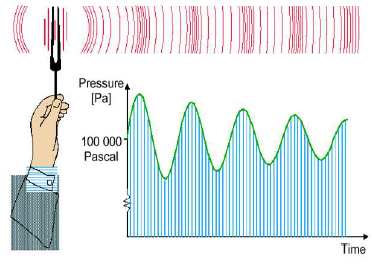
\includegraphics[scale=0.5]{acoustics/ch1/1}
	\captionof{figure}{}
	\label{fig:1.1}
	\end{wrapfigure}	
	Vibration when a mechanical excitation is applied on a material, air or water is the main source of sound. We speak about sound when the vibrations in air are perceptible by ear. The example on \autoref{fig:1.1} illustrates the vibration of a tuning fork that induces over- and under-pressure in the air around (order of magnitude small compared to ATM). Air particles are moving and describe a wave, a longitudinal wave, meaning that the particles displacement is parallel to the wave direction. Man can hear sound frequencies between 20Hz-20kHz, below we speak about infra-sound and above the limit, about ultra-sound.  
	
\section{Sound levels}
\subsection{The effective sound pressure}
	The sound perceived with a constant loudness may be both a pure sine tone and a stochastic sound generated by a source: p(t) is extremely complicated, and yet the human ear have the impression of a constant loudness. The ear seems to be sensitive to the energy of sound waves. This led to the consideration of the \textbf{effective–} or \textbf{Root-Mean-Square (RMS)} value of the sound pressure, over a (energy of sound) certain time interval, as an measure of
intensity:

	\begin{equation}
	p_{eff} = \sqrt{\frac{1}{t_2 - t_1} \int _{t_1}^{t_2}p^2(t) \, dt}.
	\end{equation}
	
\subsection{The dB-scale}
	\begin{wrapfigure}[9]{r}{6.5cm}
	\vspace{-6mm}
	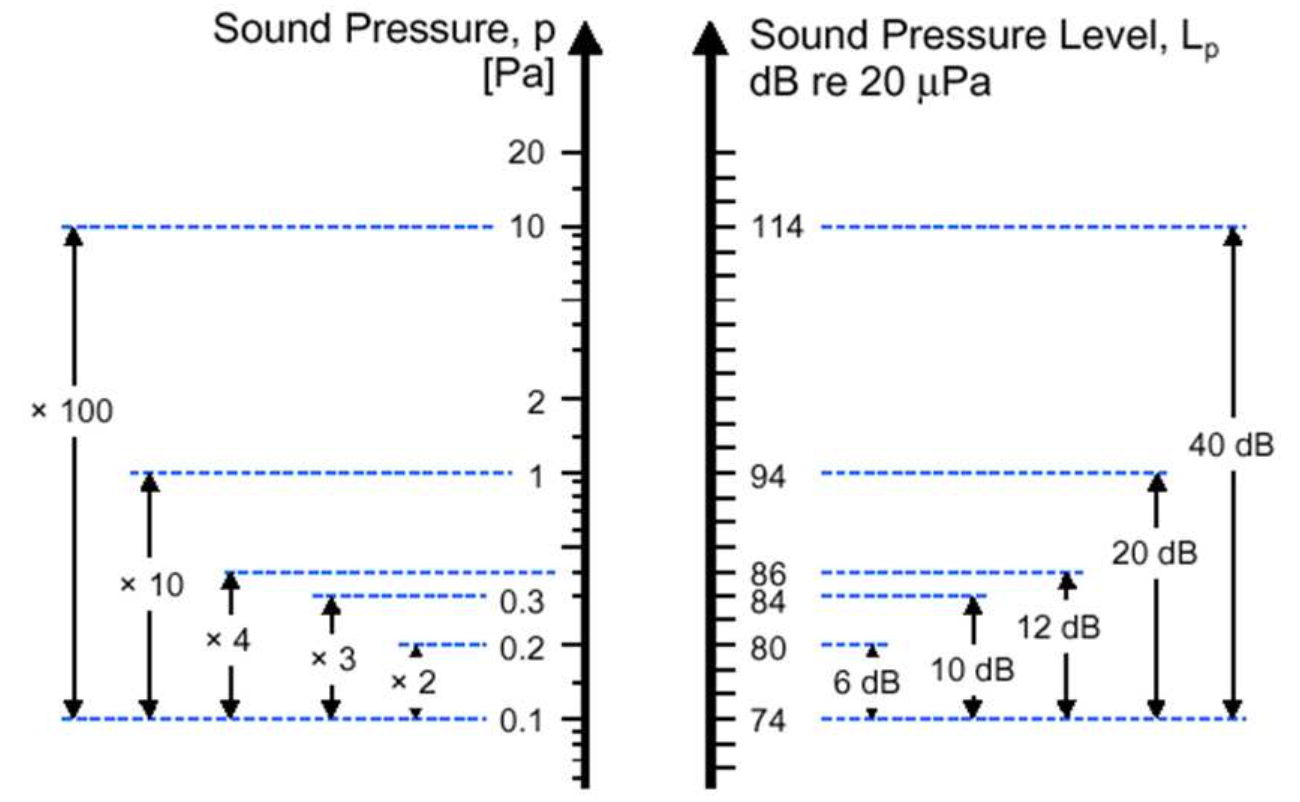
\includegraphics[scale=0.3]{acoustics/ch1/2}
	\captionof{figure}{}
	\label{fig:1.2}
	\end{wrapfigure}	
	It's another way to describe sound intensity. We define the \textbf{sound pressure level (SPL)} as:
	
	\begin{equation}
	L_p = 20 \log \frac{p}{p_0}
	\end{equation}
	
	where $p_0 = 20\mu Pa$ (threshold of human hearing). Note that every time we multiply the pressure by 10 we are in fact adding 20dB. \autoref{fig:1.2} regroups the tricks to use. 
	
	\begin{wrapfigure}[12]{l}{8cm}
	\vspace{-5mm}
	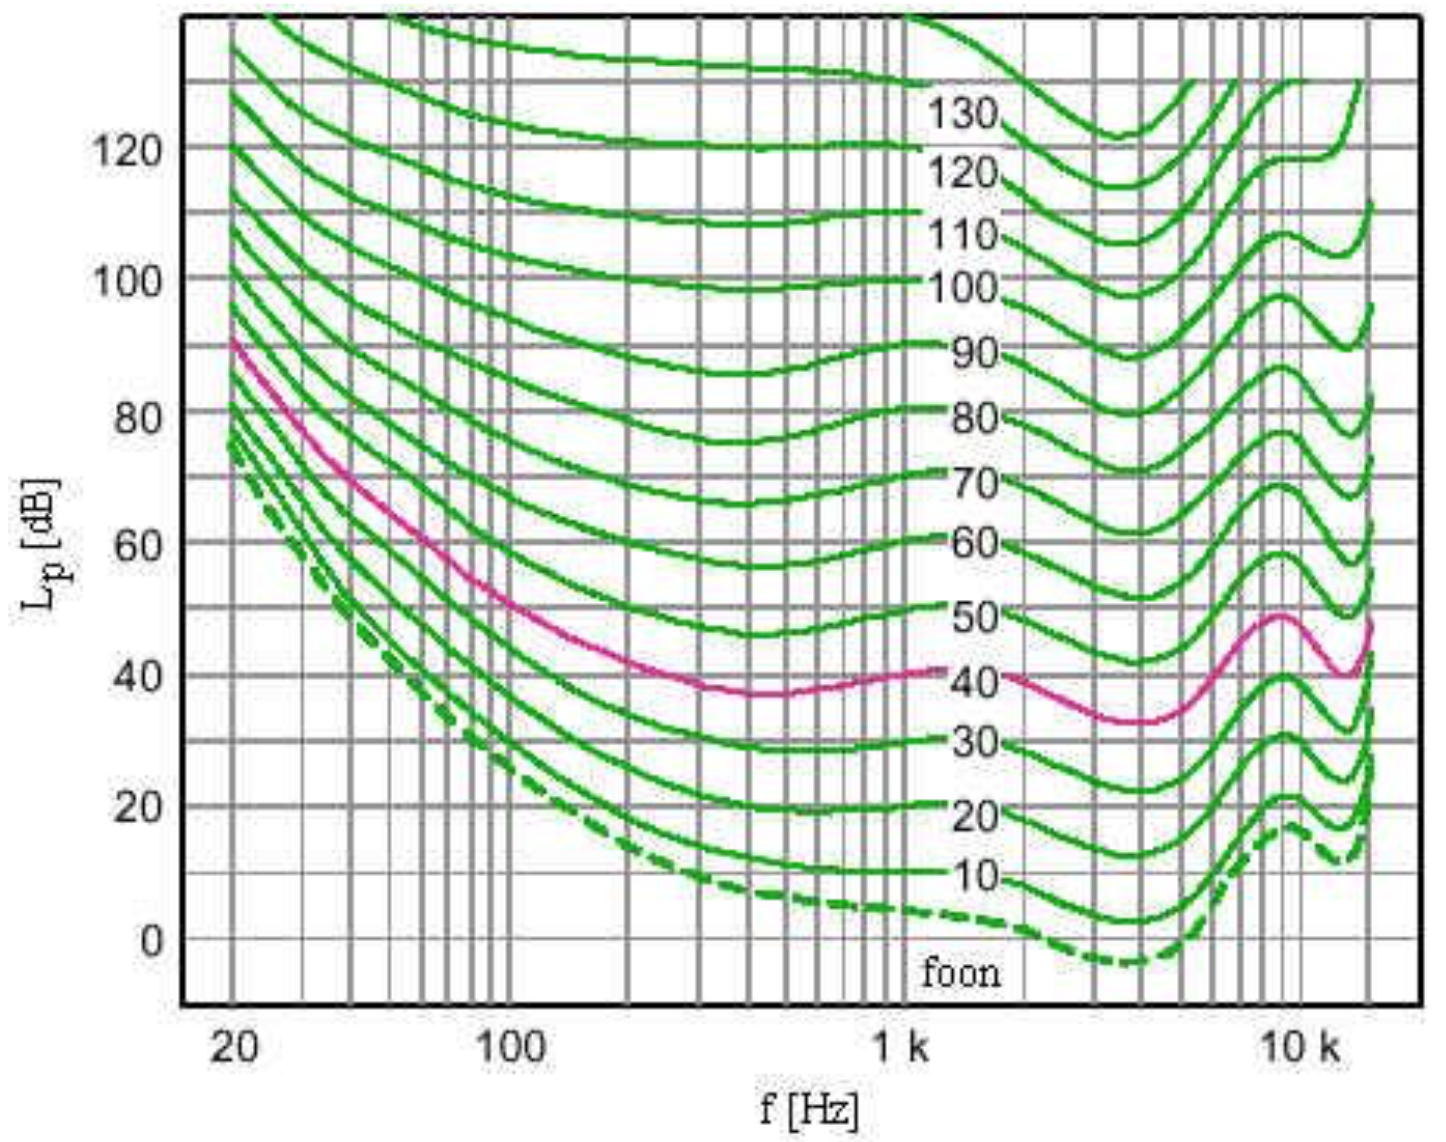
\includegraphics[scale=0.3]{acoustics/ch1/3}
	\captionof{figure}{}
	\label{fig:1.3}
	\end{wrapfigure}	
	We are expecting for example if the loudness increases of 20dB we will perceive a sound 10 times louder. But this is not the case. \autoref{fig:1.3} gives the \textbf{sensibility} in function of the frequency. We can see that as the most important for human is to communicate by language, the sensibility is higher after 200Hz. 
	
\subsection{Superposition of two sounds}
	Imagine first that we have to same sources producing a certain amount of sound, how can we compute the total amount of dB? The basic formula is: 
	
	\begin{equation}
	L_p = 10 \log \left( 10^{L_{p_1/10}} + 10^{L_{p_2}/10} \right). 
	\end{equation}
	
	\begin{wrapfigure}[4]{r}{9cm}
	\vspace{-5mm}
	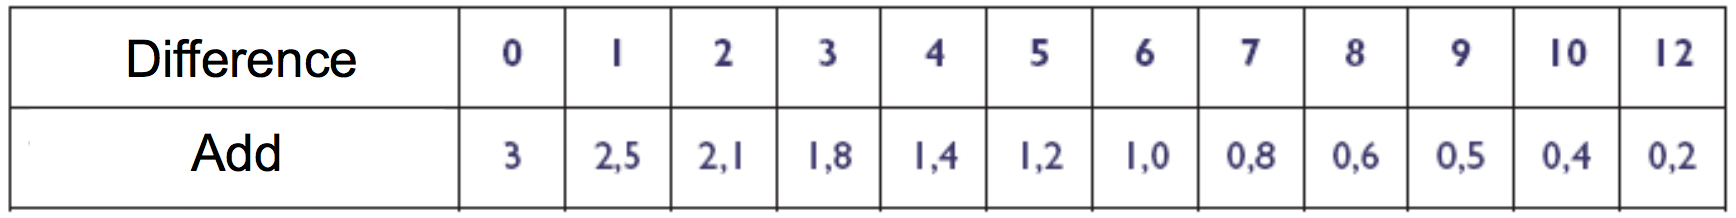
\includegraphics[scale=0.28]{acoustics/ch1/4}
	\captionof{figure}{}
	\label{fig:1.4}
	\end{wrapfigure}
	\autoref{fig:1.4}	regroups some results we can use. But we made the assumption here that we are not in phase or anti-phase. Indeed imagine that we are in phase, in this case the constructive relationship will make the pressure difference double (for example: 2 sources of 80dB in phase $\rightarrow$ pressure of 2Pa becomes 4Pa and so we add 6dB (Pa x2 = + 6dB). In fact the general formula is:
	
	\begin{equation}
	p_{rms}^2 =\frac{1}{T} \int _0^T (p_1 + p_2)^2 \, dt. 
	\end{equation}
	
	If we consider the two pressure as waves defined by amplitudes, frequencies and phases: $p_1 = Re[P_1 e^{i(\omega _1 t + \phi _1)}], p_2 = Re[P_2 e^{i(\omega _2 t + \phi _2)}]$, we have a smart way to compute this:
	
	\begin{equation}
	p_{rms}^2 = \frac{P_1^2 + P_2^2}{2} + P_1 P_2 \cos (\phi _1 + \phi _2).
	\label{eq:1.5}
	\end{equation}
	
	If the last term $P_1 P_2 \cos (\phi _1 + \phi _2) = 0$, we speak about \textbf{incoherent sources}. In this case we are computing the so known signal addition formula: RMS(total sound)$^2$ = RMS(source1)$^2$ + RMS(source2)$^2$. If the last term is $\neq 0$, the sources are \textbf{coherent} and we have to use the definition \eqref{eq:1.5}.
	
\section{Sound waves}
	\begin{wrapfigure}[5]{l}{6cm}
	\vspace{-5mm}
	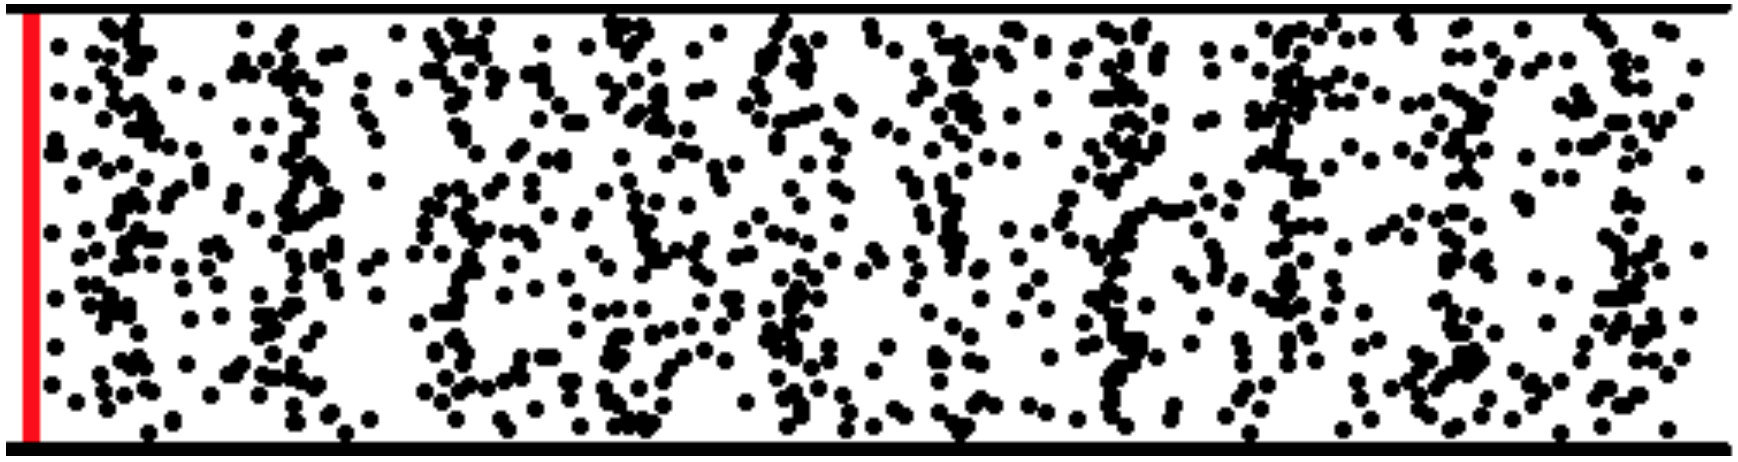
\includegraphics[scale=0.18]{acoustics/ch1/5}
	\captionof{figure}{}
	\label{fig:1.5}
	\end{wrapfigure}
	How does the sound propagates? Let's assume that we have a vibration, then the air particles in contact with the membrane are moved, that movement is then transmitted to neighboring particles. The pressure is transmitted but it is decreasing. It is decreasing because we have conversion of the energy into heat (absorption of air). The wave equation and its solution are: 
	
	\begin{equation}
	\frac{\D ^2 u}{\D x^2} = \frac{1}{c^2} \frac{\D ^2 u}{\D t^2} \qquad u(t,x) = Re\left( U_0 e^{i\omega t} e^{-i\frac{x}{c}i\omega} \right)
	\end{equation}
	
	The first exponential contains the pulsation frequency (we look the wave freezed on a point of the environment), and if we freeze and look to the shape we have the space dependence that is described by the second exponential. The wave-number , the wavelength and the speed of sound respect these relations: 
	
	\begin{equation}
	k = \frac{2\pi}{\lambda}= \frac{\omega}{c} \qquad f\lambda = c \qquad c = \sqrt{\gamma RT}. 
	\end{equation}
	
	\begin{wrapfigure}[6]{l}{4cm}
	\vspace{-5mm}
	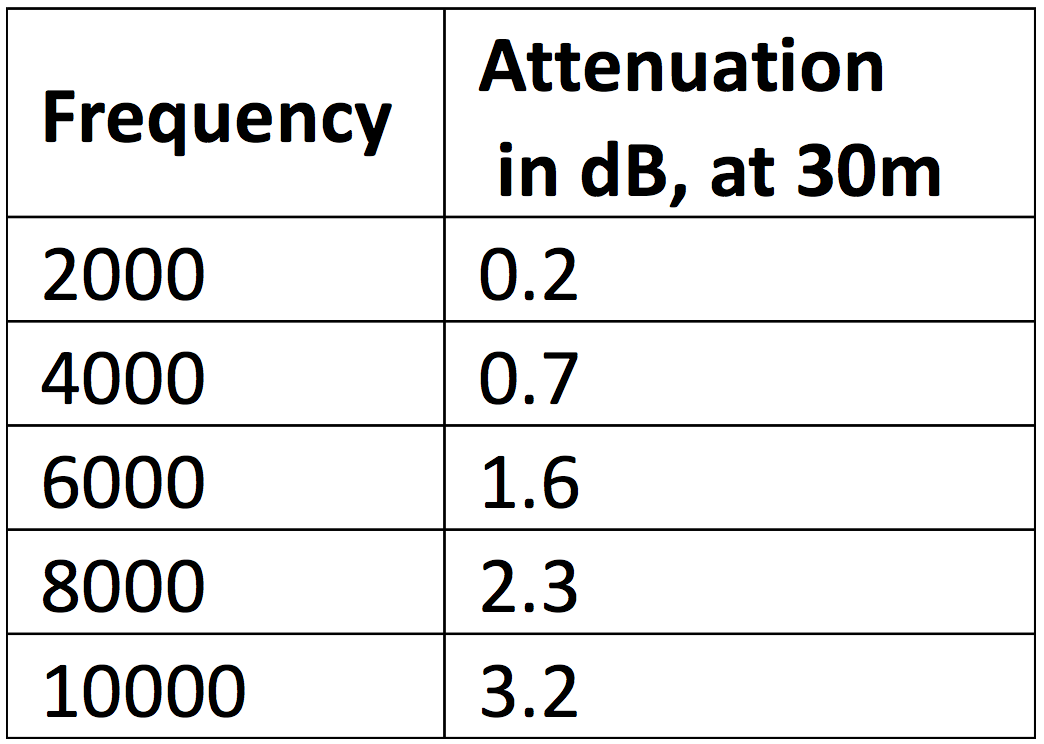
\includegraphics[scale=0.2]{acoustics/ch1/6}
	\captionof{figure}{}
	\label{fig:1.6}
	\end{wrapfigure}
	The loss depends on the frequency, the larger the wavelength the less is the attenuation. The major frequencies are below 1dB of attenuation. When we speak outdoor, the sound is not reduced because of dispersion in air, but because the energy spread in a larger space. Here is the solutions for the plane wave, the spherical wave and the cylindrical wave respectively:
	
	\begin{equation}
	p(t, x) = A e^{i\omega t} e^{-ikx} \qquad p(t, r) = \frac{A}{r} e^{i\omega t} e^{-ikr} \qquad p(t, r) = \frac{A}{\sqrt{r}} e^{i\omega t} e^{-ikr}.
	\end{equation}
	
	\begin{wrapfigure}[7]{r}{4cm}
	\vspace{-5mm}
	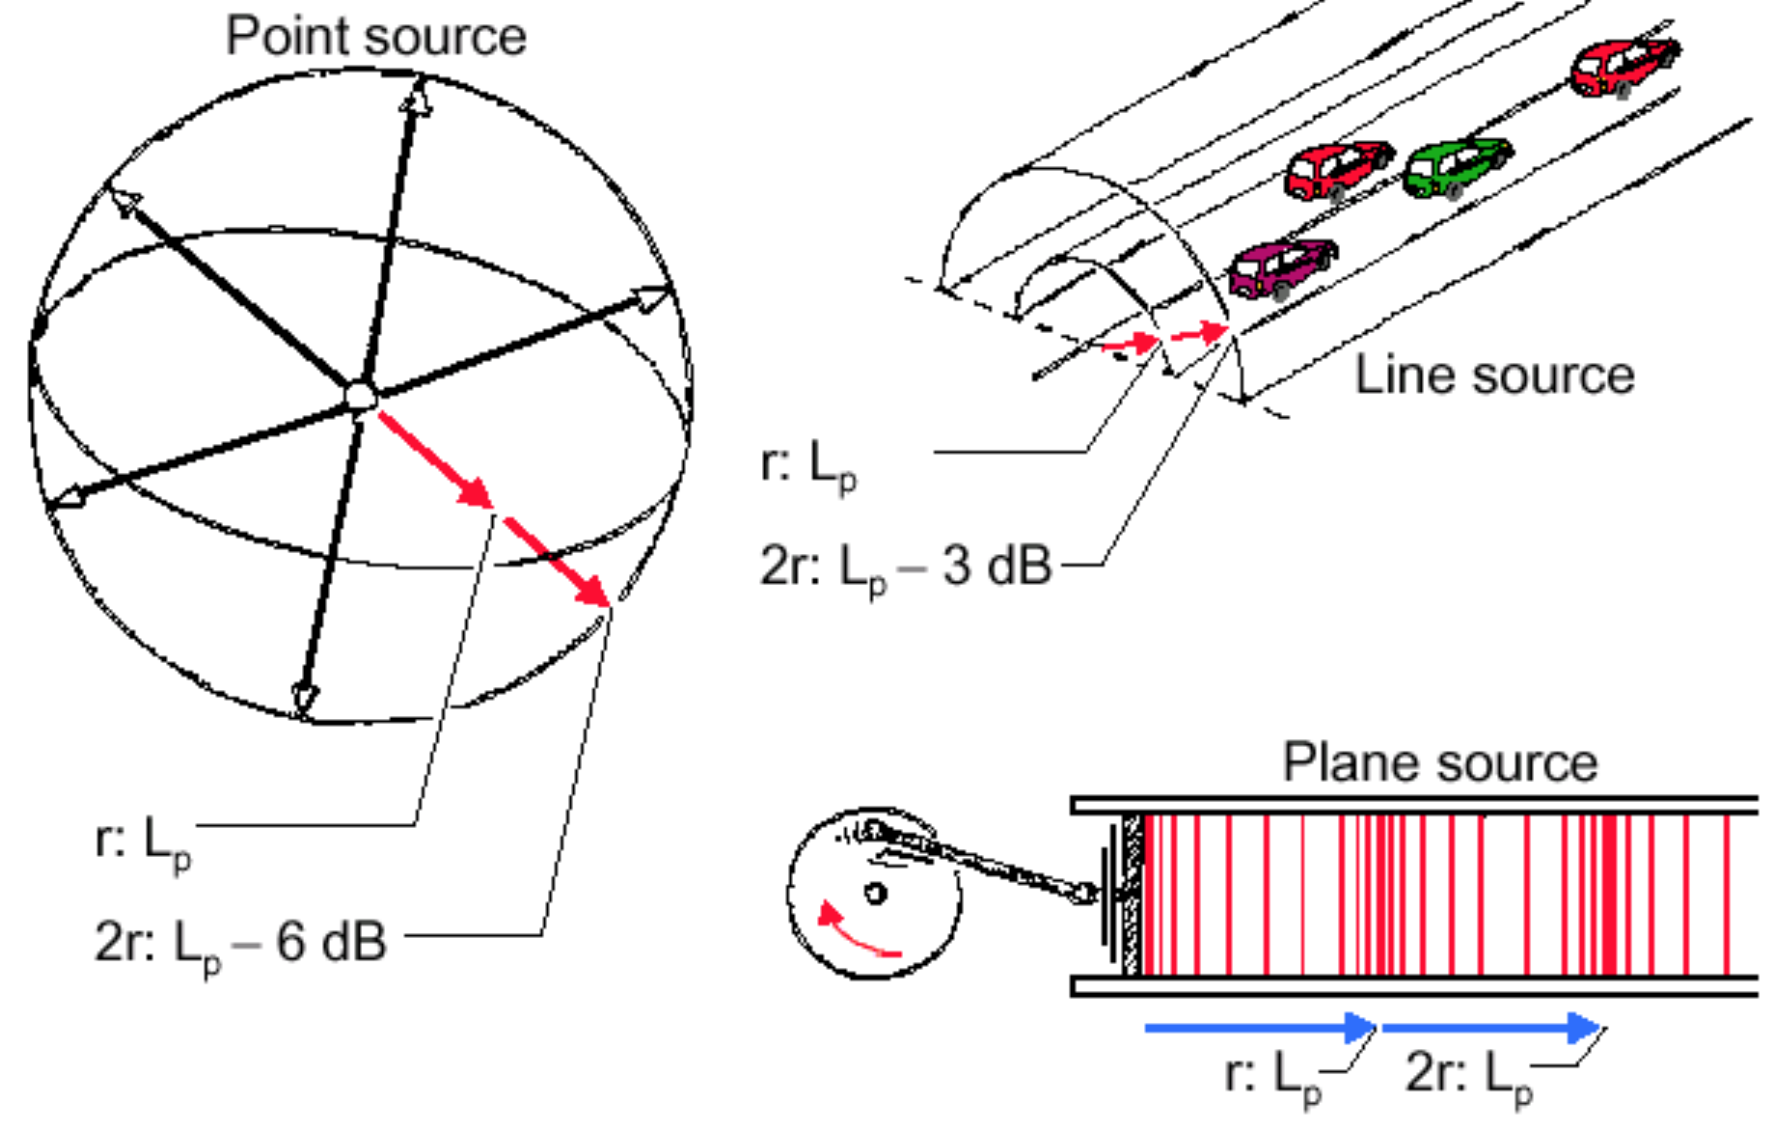
\includegraphics[scale=0.15]{acoustics/ch1/7}
	\captionof{figure}{}
	\label{fig:1.7}
	\end{wrapfigure}
	They only differ from the amplitude. We can see that if the distance double for the two last cases the sound will respectively decrease of 6dB and 3 dB ($20\log 2\approx 3$):
	
	\begin{equation}
	20\log \frac{A}{r} = 20 \log A - 20 \log r \qquad 20\log \frac{A}{\sqrt{r}} = 20 \log A - 10 \log r
	\end{equation}
	
	This is summarized on \autoref{fig:1.7}.
	
\section{Sound power}
\subsection{Sound power in Watt}
	We introduced $L_p = 20 \log p/p_0$. We concluded that this was not a good thing to define the sound radiation because of the dependency in distance. We use for this the watt which defines the \textbf{energy flux through a closed surface}. We introduce also a $L_w$ in dB:
	
	\begin{equation}
	L_w = 10\log \frac{W}{W_0}
	\end{equation}	 
	
	where $W_0 = 10^{-12}$ Watt.
	
\subsection{Sound intensity}
	This is the equivalent of the energy flux through a 1m$^2$ surface, the power per m$^2$. Here also we define a $L_I$:
	
	\begin{equation}
	L_I = 10\log \frac{I}{I_0} \qquad and \qquad W = \int _S I.dS
	\end{equation}
	
	where $I_0 = 10^{-12}$ Watt/m$^2$. 	Let's compute the instantaneous intensity: 
	
	\begin{equation}
	I_{r,inst} = \frac{dE_r}{dt dS} = \frac{F_t dr}{dt dS} = \frac{p_t dS dr}{dt dS} = p_t v_r.
	\end{equation}
	
	If we try to specify the mean intensity for plane waves, we know that we have the relationship $p/v = \rho c$:
	
	\begin{equation}
	I_r = \overline{pv_r} = p_{eff} v_{eff} = \frac{p^2_{eff}}{\rho c} = \rho c v_{eff}^2.
	\end{equation}
	
	We have to realize that this is only applicable for plane waves. There is a difference between the sound intensity and sound pressure. The pressure is a scalar value, while v is a vector, there is so a direction of propagation. 

\subsection{Relationship between sound power and sound pressure}	
	If I have a uniform sound wave we have $W=IS$, and far away from a source, we can assume the sound-wave to be planar: 
	
	\begin{equation}
	W = \frac{p^2_{eff} 4\pi r^2}{\rho c} \qquad p_{eff} = \sqrt{\frac{\rho c W}{4\pi r^2}}.
	\end{equation}
	
	This allows us to assume that in air and in ground respectively:
	
	\begin{equation}
	L_p = L_W - 10\log (4\pi r^2) \qquad and \qquad L_p = L_W - 10\log (2\pi r^2).
	\end{equation}
